\chapter{Quantum Optimal Control Theory}
The fundamental problem of Quantum Optimal Control Theory is to steer the dynamics of a quantum system in a desired way through external fields \cite{Rice2000,Shapiro2003}. Often, the goal is the transfer from an initial state, $\ket{\psi_0}$, to a desired target-state, $\ket{\psi_{\mathrm{target}}}$. The fields responsible for controlling the dynamics of the system are parametrized by a set of control parameters or functions. Optimal control theory determines the parameters, which lead to the desired dynamics of the system \cite{Werschnik2007}.\\ 
In control problems, the Hamiltonian of the system is given as
\begin{equation}
	\hat{H} =  \hat{H}_0 + \sum_{n = 1}^{m}  \hat{H}_n (u_n(t)) \; ,
	\label{eq:ControlHamiltonians}
\end{equation} 
where $\hat{H}_0$ is an uncontrollable drift, $\hat{H}_n$ are the controllable fields, and $u_n(t)$ are the control functions. A quantum system is completely controllable if every unitary operator, $\hat{U}$, is accessible from the identity operator, $\hat{I}$, via a path $\gamma (t) = \hat{U}(t, t_0)$ satisfying \cite{Schirmer2001}
\begin{equation}
	i \partial_t \hat{U}(t, t_0) = \hat{H} \hat{U}(t, t_0) \; .
\end{equation} 
For an $N$-dimensional Hilbert space, a sufficient condition for complete controllability of a quantum system is that the Lie algebra generated by the Hamiltonians in eq. \eqref{eq:ControlHamiltonians},
\begin{equation}
	L_0 = \mathrm{Lie} \left( i \hat{H}_0, i \hat{H}_1 , \ldots , i \hat{H}_m \right) \; ,
\end{equation}
is of dimension $N^2$ \cite{Ramakrishna1995}.\\
Extending these conditions to infinite-dimensional Hilbert spaces and constrained controls is non-trivial \cite{Huang1983}.


\section{The Gradient-Ascent Pulse Engineering Method - GRAPE} \label{sec:GRAPE}
The control problem presented in this thesis is steering the system from an initial state in the superfluid phase to a target-state in the Mott-Insulator phase. This is achieved by varying the lattice depth, which therefore can be considered the control parameter.\\
The optimal control problem can be stated as follows: 
Suppose the system is initially described by the state $\ket{\psi_0} = \ket{\psi (0)}$, and the potential is varied in the time interval $[ 0 , T]$. The goal is finding the set of control parameters, $\boldsymbol{u}(t)$, which brings the initial state as close as possible to the target-state, $\ket{\psi_{\mathrm{target}}}$. This is expressed in terms of a cost function
\begin{equation}
	J_T = \frac{1}{2} \left( 1-|\braket{\psi_{\mathrm{target}} | \psi (T)}|^2 \right) \; ,
	\label{eq:infidelityCost}
\end{equation}
which is given as half the infidelity between the target and the state at $t=T$. The cost function becomes zero, when the terminal state matches the target state up to an arbitrary phase. Hence, the optimal control problem can be formulated as a minimization problem of eq. \eqref{eq:infidelityCost} \cite{Jager2014}.\\
Large variations in the control parameter is often hard to achieve experimentally. Therefore, an extra term is added to the cost function, which penalizes strong variations in the control. The new cost function reads
\begin{equation}
	J = J_T + J_R = J_T + \frac{\gamma}{2} \sum_{n=1}^{m} \int_{0}^{T} \left( \pdv{u_n}{t} \right)^2 \mathrm{d}t \; ,
	\label{eq:grapeCost}
\end{equation}
where $\gamma$ weighs the relative importance between matching states and smoothness of the control \cite{Jager2014}. As the state transfer is considered the highest priority, $\gamma \ll 1$ such that $J_T$ dominates the cost function of eq. \eqref{eq:grapeCost}.\\

A powerful way of performing optimal control is the Gradient-Ascent Pulse Engineering (GRAPE) method. Through GRAPE, the gradient of the cost function \eqref{eq:grapeCost} can be evaluated and used to update the existing set of controls \cite{Khaneja2005}. Thereby, one achieves an optimization of the cost function.\\
The gradient of the cost function can be derived in multiple ways. A common method is introducing a Lagrange multiplier \cite{Hohenester2007, Winckel2008, BECcontrol}, which forces the dynamics to obey the Schrödinger equations. This method considers the states and the control as continuous functions, which must be discretized after the derivation of the gradient for numerical purposes. However, postponing the discretization until the very last step causes a loss of accuracy, as a series of higher order corrections due to the discretization are lost.
Here, an alternative derivation following \cite{Khaneja2005, deFouquieres2011} is presented in which the discretization is introduced immediately. \\
Assume the transfer time, $T$, is discretized in steps of $\Delta t = T/N$. Subjecting the control to a similar discretized yields
\begin{equation}
	u_n = \left( u_n (t_1) , \ldots , u_n (t_N)  \right)  \; .
\end{equation}
The time-evolution of the system during the time step $j$ is given by the propagator
\begin{equation}
	\hat{\mathcal{U}}_j \equiv \hat{\mathcal{U}} (u(t_j)) = \exp \bigg\{ -i \left(  \sum_{n = 1}^{m}  \hat{H}_n (u_n(t_j))  \right) \Delta t \bigg\} \; . 
\end{equation} 
Thereby, the cost function \eqref{eq:grapeCost} becomes
\begin{equation}
	J = \frac{1}{2} \left( 1 - |\braket{\psi_{\mathrm{target}} | \prod_{j = 1}^{N} \hat{\mathcal{U}}_j | \psi (0)}|^2 \right) + \frac{\gamma}{2} \sum_{n = 1}^{m} \sum_{j = 1}^{N-1} \left( \frac{\Delta u_n (t_j)}{\Delta t} \right)^2 \Delta t \; ,
	\label{eq:discreteCost}
\end{equation}
where $\Delta u_n (t_j) =  u_n (t_{j+1}) - u_n (t_j)$. The full gradient of the cost, $\nabla J(\boldsymbol{u})$, is a vector of partial derivatives $\frac{\partial J(\boldsymbol{u})}{\partial u_n (t_j)}$, which can be derived analytically.\\
First, consider the derivative of the regularization
\begin{align}
	\frac{\partial J_R}{\partial u_n (t_j)} &= \frac{\gamma}{2} \left( 2 \frac{u_n (t_j) - u_n (t_{j-1})}{\Delta t^2} - 2 \frac{u_n (t_{j+1}) - u_n (t_j)}{\Delta t^2} \right) \Delta t \nonumber \\
	&= \frac{\gamma}{\Delta t} \left( 2 u_n (t_j) - u_n (t_{j+1}) - u_n (t_{j-1}) \right) \; . \label{eq:regularizationGrad}
\end{align}
The part of the gradient related to the regularization depends only on the control, whereby it can be calculated without considering the state of the system.\\ 
Next, consider the derivative of $J_T$. Defining the transfer probability amplitude $\tau \equiv \braket{\psi_{\mathrm{target}} | \psi (T)}$, the derivative of the final infidelity with respect to the control can be written as 
\begin{equation}
	\frac{\partial J_T}{\partial u_n (t_j)} = - \frac{1}{2} \frac{\partial}{\partial u_n (t_j)}  \tau^* \tau   = - \Re \left( \tau^* \frac{\partial \tau}{\partial u_n (t_j)} \right) \; .
	\label{eq:dJTdu}
\end{equation}
From eq. \eqref{eq:dJTdu} it is evident that the derivative of the infidelity depends only on the derivative of the transfer probability amplitude, $\frac{\partial \tau}{\partial u_n (t_j)}$. This derivative can be rewritten as
\begin{align}
	\frac{\partial \tau}{\partial u_n (t_j)} &= \frac{\partial }{\partial u_n (t_j)} \Braket{\psi_{\mathrm{target}} | \prod_{j = 1}^{N} \hat{\mathcal{U}}_j | \psi (0)} \nonumber \\
	&= \Braket{\psi_{\mathrm{target}} | \hat{\mathcal{U}}_N \ldots \hat{\mathcal{U}}_{j+1} \frac{\partial \hat{\mathcal{U}}_{j}}{\partial u_n (t_j)} \hat{\mathcal{U}}_{j-1} \ldots \hat{\mathcal{U}}_{1} | \psi (0)}
	\label{eq:dcdu}
\end{align}
Multiplying eq. \eqref{eq:dcdu} with $\tau^*$ to recreate the result of eq. \eqref{eq:dJTdu} yields
\begin{align}
	\tau^* \frac{\partial \tau}{\partial u_n (t_j)} &=  \braket{\psi(T) | \psi_{\mathrm{target}}} \Braket{\psi_{\mathrm{target}} | \prod_{j' = j +1}^{N} \hat{\mathcal{U}}_{j '} \frac{\partial \hat{\mathcal{U}}_{j}}{\partial u_n (t_j)} \prod_{j' = 1}^{ j-1} \hat{\mathcal{U}}_{j '} | \psi (0)} \\
	&= i \Braket{\chi (T) | \prod_{j' = j +1}^{M} \hat{\mathcal{U}}_{j '} \frac{\partial \hat{\mathcal{U}}_{j}}{\partial u_n (t_j)} \prod_{j' = 1}^{ j-1} \hat{\mathcal{U}}_{j '} | \psi (0)} \\
	&= i \Braket{\chi (t_j) |  \frac{\partial \hat{\mathcal{U}}_{j}}{\partial u_n (t_j)} | \psi (t_{j-1})} \; ,
	\label{eq:gradientForBack}
\end{align}
where $\ket{\chi (T)} \equiv i \ket{\psi_{\mathrm{target}}} \braket{\psi_{\mathrm{target}} | \psi (T)}$ is the projection of the final state unto the target state. Notice how in eq. \eqref{eq:gradientForBack} the state $\ket{\chi (T)}$ has been propagated backwards in time.\\ 
The derivative of the propagator, $\hat{\mathcal{U}}_{j}$, is non-trivial, due to possible non-commutativity between the Hamiltonian and its derivative. This results in a series of higher order corrections to the derivative of propagator.
Expanding the propagator as a Taylor series before taking the derivative gives
\begin{align}
	\frac{\partial \hat{\mathcal{U}}_{j}}{\partial u_n (t_j)} &= \frac{\partial}{\partial u_n (t_j)}  \exp \left( -i \hat{H} \Delta t \right) \nonumber \\
	&= \sum_{p = 0}^{\infty} \frac{( -i \Delta t  )^p}{p!} \frac{\partial \hat{H}^p}{\partial u_n (t_j)} \; .  
	\label{eq:derivTaylorExp}
\end{align}
As mentioned before the Hamiltonian may not commute with its derivative. Therefore, one must be careful when taking the derivative of $\hat{H}^p$. Retaining the ordering of the operators while taking the derivative yields
\begin{align}
	\frac{\partial \hat{\mathcal{U}}_{j}}{\partial u_n (t_j)} &= \sum_{p=1}^{\infty} \frac{ \left( -i \Delta t \right) ^p }{p!} \sum_{q=0}^{p-1} \hat{H}^q \frac{\partial \hat{H}}{\partial u_n (j)} \hat{H}^{p-q-1} \nonumber \\
	&= \sum_{p=0}^{\infty} \sum_{q=0}^{\infty} \frac{A^p B A^q}{(p+q+1)!} \; , \label{eq:derivTaylorExp2}
\end{align} 
where $A \equiv -i \hat{H} \Delta t$ and $B \equiv -i \partial \hat{H}/\partial u_n (t_j) \Delta t$ have been defined for notational convenience. Through the standard relations of the gamma function, $\Gamma (z)$, one can derive the identity
\begin{equation}
	\frac{1}{(p+q+1)!} = \frac{1}{p! q !} \int_{0}^{1} (1-\alpha)^p \alpha^q \mathrm{d}\alpha \; .
\end{equation}
Thereby eq. \eqref{eq:derivTaylorExp2} can be expressed as
\begin{align}
	\frac{\partial \hat{\mathcal{U}}_{j}}{\partial u_n (t_j)} &= \sum_{p=0}^{\infty} \sum_{q=0}^{\infty} \frac{A^p B A^q}{p! q !}  \int_{0}^{1} (1-\alpha)^p \alpha^q \mathrm{d}\alpha \nonumber \\
	&= \int_{0}^{1} \sum_{p=0}^{\infty} \sum_{q=0}^{\infty} \frac{(A (1- \alpha))^p}{p!} B \frac{(A \alpha)^q}{q!}  \mathrm{d}\alpha \nonumber \\
	&= \int_{0}^{1} e^{ (1- \alpha) A} B e^{ \alpha A} \mathrm{d}\alpha \nonumber \\
	 &= e^A \int_{0}^{1} e^{ - \alpha A} B e^{ \alpha A} \mathrm{d}\alpha \; , \label{eq:eq:derivTaylorExp3}
\end{align}
where the expansion of the exponential function has been used to eliminate the sums. Although eq. \eqref{eq:eq:derivTaylorExp3} looks rather simple, evaluating the integral in its current form is a fairly hard task. Instead, the integral can be explicitly solved by applying the Baker–Campbell–Hausdorff expansion 
\begin{equation}
	e^X Y e^{-X} = \sum_{k = 0}^{\infty} \frac{ [ X,Y  ]_k }{k!} = Y + [ X,Y  ] + \frac{1}{2!} [ X , [ X,Y  ]] + \frac{1}{3!} [X, [ X , [ X,Y  ]]  ] + ...
\end{equation}
where $[ X , Y ]_k = [ X ,[ X , Y]]_{k-1}$ and $[X,Y]_0 = Y$ is the definition of the recursive commutator \cite{Wilcox1967}. Thus, eq. \eqref{eq:eq:derivTaylorExp3} reads
\begin{align}
	\frac{\partial \hat{\mathcal{U}}_{j}}{\partial u_n (t_j)} &=  e^A \int_{0}^{1} \sum_{k = 0}^{\infty } \alpha^{k} \frac{(-1)^k}{k!} [ A,B  ]_k \mathrm{d}\alpha \nonumber \\
	&= e^A  \sum_{k = 0}^{\infty }  \frac{(-1)^k}{(k+1)!} [ A,B  ]_k \; .
\end{align}
Inserting this final expression for the derivative of the propagator into eq. \eqref{eq:dJTdu}, one finds the exact derivative of the infidelity 
\begin{align}
\frac{\partial J_T}{\partial u_n (t_j)} &=  - \Re  \Braket{\chi (t_j) | i e^{-i \hat{H} \Delta t}  \sum_{k = 0}^{\infty }  \frac{(-1)^k}{(k+1)!} \left[ -i \hat{H} \Delta t , -i \frac{\partial \hat{H}}{\partial u_n (t_j)} \Delta t  \right]_k | \psi (t_{j-1})}  \nonumber \\
	&=  - \Re  \Braket{\chi (t_{j-1}) | \sum_{k = 0}^{\infty }  \frac{i^{k} \Delta t^{k+1}}{(k+1)!} \left[ \hat{H} , \frac{\partial \hat{H}}{\partial u_n (t_j)}  \right]_k | \psi (t_{j-1})}  \; . \label{eq:higherOrderGradient}
\end{align}
For small time-steps the higher order corrections can be neglected, however, choosing a larger time-step reduces the run-time of the time-evolution, which is critical when describing many-body systems. Therefore, when using large time-steps, higher-order correlations should be included to preserve accuracy. Computing the higher order corrections can be done efficiently by analytically deriving the commutators beforehand. In section \ref{sec:modTMDRG} an alternative propagator is constructed using the Suzuki-Trotter expansion, which causes the gradient to be exact to zeroth order.\\
Finally, combining the derivatives of eq. \eqref{eq:regularizationGrad} and \eqref{eq:higherOrderGradient} produces the entries of the gradient vector for the cost function
\begin{align}
	\frac{\partial J (\boldsymbol{u})}{\partial u_n (t_j)}  &= - \Re \Braket{\chi (t_{j-1}) | \left( i \frac{\partial \hat{H}}{\partial u_n (t_j)} \Delta t + \mathrm{h.o.} \right)  | \psi (t_{j-1})}  \nonumber \\
	& \quad + \frac{\gamma}{\Delta t} \left( 2 u_n (t_j) - u_n (t_{j+1}) - u_n (t_{j-1}) \right) \; .
	\label{eq:costGradient}
\end{align}
Here $\mathrm{h.o.}$ denotes all higher order terms ($k > 0$).\\ 
Through the analytically derived gradient, the cost can be iteratively updated using gradient-based optimization methods until a desired threshold is reached. This forms the framework of the Gradient-Ascent Pulse Engineering (GRAPE) algorithm \cite{Khaneja2005}, which is summarised below:

\begin{algorithm}
\begin{algorithmic}
\caption{GRAPE Algorithm}
\State Choose initial control $\boldsymbol{u}^{(1)}$.
\While{$ J > J_{\mathrm{threshold}}$}
	\State Calculate $\ket{\psi (t_k)} = \prod_{j=1}^{k} \hat{\mathcal{U}}_j \ket{\psi (0)}$ for $k = 1 \ldots N$.
	\State Calculate $\ket{\chi (t_k)} = \prod_{j=N}^{k} \hat{\mathcal{U}}_{j}^{\dag} \ket{\chi (T)}$ for $k = N \ldots 1$. 
	\State Evaluate $\frac{\partial J}{\partial u_n (t_k)}$ for $k = 1 \ldots N$ and $n = 1 \ldots m$ according to eq. \eqref{eq:costGradient}.
	\State Update controls using gradient such that $J^{(i + 1)} < J^{(i)}$. 
\EndWhile
\end{algorithmic}
\end{algorithm}
The computations are performed under the boundary conditions
\begin{align}
	\boldsymbol{u}(0) &= \text{fixed value} \label{eq:firstBound} \\
	\boldsymbol{u}(T) &= \text{fixed value} \\
	\ket{\psi (0)} &= \ket{\psi_0} \\
	\ket{\chi (T)} &= i \ket{\psi_{\mathrm{target}}} \braket{\psi_{\mathrm{target}} | \psi (T)} \; .  \label{eq:lastBound}
\end{align}
Figure \ref{fig:ControlUpdate} illustrates an update step of the controls such that the cost function is reduced.
\begin{figure}[!h]
	\centering
	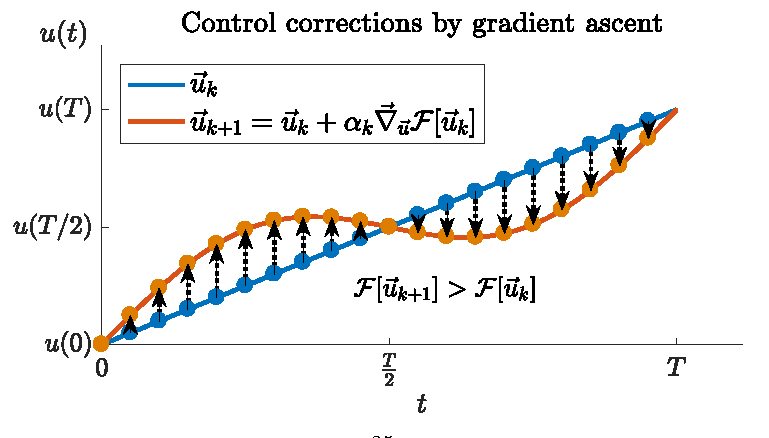
\includegraphics[width=0.7\columnwidth]{Figures/ControlUpdate.pdf} 
	\caption{ \textit{Visualisation of update step $i \to i+1$ of the control $\boldsymbol{u}^{(i)}$ resulting in a decreased cost function.}}
	\label{fig:ControlUpdate} 
\end{figure} 
Although the starting guess of the control, $\boldsymbol{u}^{(1)}$, can be completely random, both faster convergence and lower convergence value is achieved by choosing a good starting seed. Clearly, there is no guarantee that the algorithm will converge to the global optimum, as it is based on a gradient ascent procedure \cite{Khaneja2005}. Nevertheless, the algorithm can be made to search a large portion of the parameter space by executing it multiple time for various seeds.  


\section{Gradient-Optimization Using Parametrization - GROUP} \label{sec:GROUP}
The convergence rate of optimal control sequences has been shown to be greatly improved by employing gradient-based methods, such as GRAPE, for updating the control \cite{Jager2014}.
One of the disadvantages of GRAPE is the dimension for the optimization. As the duration of the control pulse is discretized into $N$ time-steps, the control at each of these steps must be optimized. For long durations or small time-steps the resulting dimension of the optimization ($N$) will be very large. One may consider this type of control parametrization having too many degrees of freedom for the optimization. 
However, employing a proper parametrization of the control can drastically reduce the optimization dimension \cite{Winckel2008}.\\
A common choice is employing a chopped basis, which parametrizes the control as
\begin{equation}
	u(t) = u_0 (t) + S(t) \sum_{n=1}^{M} c_n f_n (t) \; , \label{eq:controlParametrization}
\end{equation}   
where $f_n$ are the basis functions, and $c_n$ are the optimization coefficients. In addition, $u_0 (t)$ is the initial control function, and $S (t)$ is a shape function enforcing the boundary conditions of the control, whereby $S(0) = S(T) = 0$ CITE JJ ARTIKEL. The shape function used throughout this thesis consists of two steep sigmoids oriented such that $S$ is unit for most time steps. The basis functions, $f_n$, must be chosen based on physical insight of the system. For the control problem discussed in this thesis, employing a basis of sine functions has proven itself useful, as the sine functions are excellent at describing the smoothly varying control pulses desired CITE JJ. Thus, the basis functions read $f_n = \sin \left( \frac{\omega_n t}{T} \right)$, where $\omega_n = n \pi$.
An extension of this type of chopped basis was done in \cite{Doria2011,Caneva2011crab}, introducing random shifts to the frequencies resulting in the Chopped RAndom Basis or \textsc{CRAB}. In recent years the \textsc{CRAB} parametrization has been used together with the Nelder-Mead hill climbing algorithm to solve various control problems \cite{Doria2011,Caneva2011,FrankBloch,Lloyd2014}.\\
The great advantage of employing a reduced basis representation is the drastic reduction in the optimization space. However, artificial minima can be introduced, if the chosen basis is incapable of spanning the part of the optimization space containing the optimal solutions \cite{Rach2015}. Hence, the chopped basis dimension, $M$, must be chosen with consideration.\\

The Gradient-Optimization Using Parametrization or \textsc{GROUP} algorithm introduced in JJ CITE combines the chopped basis representation with the \textsc{GRAPE} algorithm. Parameterizing the control alters the gradient of the cost functional described in eq. \eqref{eq:costGradient}. The new gradient can be derived using the chain rule
\begin{align}
	\frac{\partial J }{\partial c_n} &= \sum_{j = 1}^{N} \frac{\partial J }{\partial u(t_j)} \frac{\partial u(t_j)}{\partial c_n} \nonumber \\
	&= \sum_{j = 1}^{N} \frac{\partial J }{\partial u(t_j)} S(t_j) f_n(t_j) \; , \label{eq:GROUPgradient} 
\end{align}
where only a single control has been chosen for cleaner notation. The gradient in \textsc{GROUP} is more complicated than in \textsc{GRAPE}. However, the cost of computing the gradient is still dominated by the evaluation of the derivative $\frac{\partial J }{\partial u(t_j)}$, as this requires two time-evolutions for the full duration, $T$. Therefore, the increased computational cost of evaluating the gradient is negligible compared to the reduced dimensionality through the parameterization. 
In JJREF a comparison between different optimization algorithms for optimal control demonstrated that \textsc{GROUP} outperformed both \textsc{GRAPE} and Nelder-Mead with \textsc{CRAB} in term of fidelity reached and number of function evaluations required for convergence.

\subsection{Alteration of constraints through GROUP}
Consider the non-parametrized optimization problem discretized in time which is subjected to the boundaries of eq. \eqref{eq:firstBound}-\eqref{eq:lastBound}. Optimal control problems are often subjected to constraints to avoid the control containing infeasible values
\begin{equation}
	 u_{min} \leq u(t_j) \leq u_{max} \; .
\end{equation}
In the case of the Bose-Hubbard model, a lower bound of the control is needed, as the model is not well defined for lattice depths well below the tight-binding limit.\\
In order to enforce the constraints during a gradient-based optimization, the derivative of the constraints are needed as well. As the problem may be subjected to multiple sets of constraints, a Jacobian matrix of the constraint derivatives must be calculated
\begin{equation}
	\boldsymbol{J}_{ij} = \frac{\partial g_i}{\partial x_j} \; ,
\end{equation}
where $g_i$ are the constraint functions, and $x_j$ are the optimization parameters.\\
Employing the GROUP algorithm causes a parametrization of the control, eq. \eqref{eq:controlParametrization}, which in turn alters the constraints. Thus, one must also consider the alteration of the Jacobian. In the Bose-Hubbard control problem the constraint function is simply the control itself, whereby the transformed Jacobian reads
\begin{equation}
	\boldsymbol{J}_{ij} = \frac{\partial u(t_i)}{\partial c_j} = S(t_i) f_j (t_i) \; . \label{eq:ConstJacobian}
\end{equation}
Thus, the Jacobian of the constraints has $N \times M$ entries, where $N$ is the number of time steps, and $M$ is the dimension of the chopped basis. The matrix elements Jacobian \ref{eq:ConstJacobian} are easy to evaluate during the optimization, as they remain constant for the entire duration.


\section{Interior Point Method} \label{sec:IntPoint}
Through the gradient of the cost functional, the control functions can be iteratively updated yielding an improved cost. The update of the control functions can be done using various hill-climbing methods.
Interior point methods are modified versions of Newtons method for bound, constrained problems. The methods approach the solution from within the feasible region and provides efficient performance while having better theoretical properties than the standard simplex method \cite{wright}.\\
For simplicity a linear version of the method will be derived, however, the formalism can easily be extended to non-linear problems \cite{wright}.

\subsection{Karush–Kuhn–Tucker conditions}
Consider the general minimization problem
 \begin{align}
	\min_{x \in \mathbb{R}^n} \;  & \; c^T x \label{eq:LinOptProb} \\
	\text{subject to} \;  & \; A x = b  \nonumber \\ 
							& \; x \geq 0 \nonumber \; ,
\end{align}
can be derived from any linear problem through slack variables, which transform inequality constraints into equality constraints at the cost of introducing extra variables \cite{ipopt}.
The Karush–Kuhn–Tucker (KKT) conditions are first-order conditions for a solution of a nonlinear problem to be an optimum. Unlike Lagrange multipliers, the KKT conditions accommodates inequality constraints.
\begin{theorem}
	Suppose that $x^*$ is a local solution of the objective function $f  :  \mathbb{R}^n \to \mathbb{R}$ with respect to a collection of constraints $\{ c_i(x)  \}_{i=1}^{m}$, where $c_i :  \mathbb{R}^n \to \mathbb{R}$. Let $\mathcal{L}$ be the Lagrangian of the problem. If the subset of the equality constraints $\{ c_i(x) \in \mathcal{E}\}$ has the property that $\{ \nabla c_i(x^*)\}$ is linear independent, then a vector of Lagrange multipliers, $\lambda^*$, exists for which the following holds:
	\begin{subequations}	
	\begin{align}
		\nabla_x \mathcal{L}(x^*,\lambda^*) &= 0 \; ,  \\
		c_i(x^*) &= 0 \; , \qquad \forall i \\
		\lambda_{i}^* &\geq 0 \; , \qquad \forall i \in \mathcal{I} \\
		\lambda_{i}^* c_i(x^*) &= 0 \; , \qquad \forall i \in \mathcal{E} \cup \mathcal{I}
	\end{align}
	\end{subequations}	
	where $\mathcal{E}$ and $\mathcal{I}$ denote the equality and inequality subspaces respectively \cite{wright}.  
\end{theorem}
If $x^*$ satisfies the conditions, its objective value must be at an optimum point.


\subsection{Barrier Problems}
In interior point methods the boundaries of the variables are enforced through a barrier function, which keeps the objective function continuously differentiable.
A general, linear optimization problem can be associated with a barrier function
\begin{equation}
	B(x , \mu) = c^T x - \mu \sum_{i=1}^{n} \ln x_i \; ,
\end{equation} 
where $\mu > 0$ is the barrier parameter. For $\mu \to 0$ one recovers the original problem \eqref{eq:LinOptProb}.
The optimization Lagrangian of the barrier problem is
\begin{equation}
	\mathcal{L}(x, \lambda, s) = c^T x - \mu \sum_{i=1}^{n} \ln x_i - \lambda^T (A x -b) \; ,
\end{equation}
where $\lambda \in \mathbb{R}^m$ is the Lagrange multiplier for the $A x = b$ constraint. Now, let $X = \mathrm{Diag}(x_1 , \ldots , x_n)$, $e = (1,1, \ldots , 1)^T$, $s = \mu X^{-1} e$, and $S = \mathrm{Diag}(s_1 , \ldots , s_n)$. Thereby the KKT conditions of the barrier problem can be stated as 
\begin{subequations}
\begin{align}
	A^T \lambda + s &= c \\
	A x &= b \\
	X S e &= \mu e \; .
\end{align}
\end{subequations}
By adding the barrier term the KKT conditions has been "relaxed", as they are no longer zero \cite{ipnote}. Again, for $\mu \to 0$ the original conditions are recovered. 


\subsection{Primal-Dual Interior Point Method}
Primal-dual methods optimize an additional, \textit{dual}, problem while optimizing the main, \textit{primal}, problem.
Consider the initial linear problem \eqref{eq:LinOptProb}, whose dual is given by 
\begin{align*}
	\max_{\lambda \in \mathbb{R}^n} \;  & \; b^T \lambda \\
	\text{subject to} \;  & \; A^T \lambda + s = c  \\
							& \; s \geq 0 \; .
\end{align*}
The two problems are closely related. If either the primal or the dual problem has a solution, then so does the other, and the objective values are equal. If either problem is unbounded, then the other problem is infeasible. If a solution exists, then the optimal solution to the dual problem are the Lagrange multipliers to the primal problem and vice versa \cite{wright}.
Hence, for primal-dual algorithms triplet of variables, $(x , \lambda , s)$, is considered when computing the optimum of a function. Note, the dual of the dual problem is the original problem.\\

The primal-dual interior point method optimizes a subproblem for a given $\mu$ by taking taking constrained Newton steps towards the optimum \cite{wright}. The optimal solution of the main problem is found by solving these subproblems iteratively for ever decreasing $\mu$ using the previous solution as starting point \cite{ipopt}.\\
The solutions for the primal-dual subproblems are characterized by the KKT conditions, which can be written into a single mapping
\begin{align}
    F(x , \lambda, s) &= \begin{pmatrix}
           A^T \lambda + s - c \\
           A x - b \\
           X S e
         \end{pmatrix} = 0
\end{align}
with the Jacobian
\begin{align}
    J(x , \lambda, s) = \begin{pmatrix}
           0 & A^T & I	\\
           A & 0 & 0 	\\
           S & 0 & X
         \end{pmatrix}
\end{align}
The Newton direction, $(x_B , \lambda_B , s_B)$, can be written as the solution to the system of equations
\begin{align}
J \begin{pmatrix}
           x_B \\
           \lambda_B \\
           s_B
         \end{pmatrix} = -F \label{eq:StepDir}
\end{align}
The step direction equation \eqref{eq:StepDir} does not take the barrier term into account. However, the constraints can easily be added to the problem, as the barrier term merely alters the KKT conditions, $F$. Thereby, the constrained Newton step for the primal-dual problem reads
\begin{align}
	\begin{pmatrix}
    	 0 & A^T & I    \\
         A & 0 & 0 		\\
         S & 0 & X
    \end{pmatrix} 
    \begin{pmatrix}
    	x_b 		    \\
        \lambda_B		\\
        s_B
    \end{pmatrix} =
    - \begin{pmatrix}
    	  A^T \lambda + s - c 	\\
          A x - b 				\\
          X S e - \mu e
    \end{pmatrix} \; . \label{eq:newtondirection}
\end{align}
The functions are optimized by taking a step of length $\alpha$ in the direction specified by eq. \eqref{eq:newtondirection}, such that the updated function values read
\begin{equation}
	(x_{k+1} , \lambda_{k+1} , s _{k+1}) = (x_{k} , \lambda_{k} , s _{k}) + \alpha  (x_B , \lambda_B , s_B) \; , \label{eq:newtonstep}
\end{equation}
where $\alpha$ can be found using a line-search or other more sophisticated methods.
The procedure above can be summarized in the following algorithm \cite{ipnote}:\\
\begin{algorithm}
\begin{algorithmic}
\caption{Primal-Dual Interior Point Method}
\State Choose $\sigma \in (0,1)$ and $\mu_0 > 0$.
\State Choose initial point $(x_0 , \lambda_0 , s_0)$ within feasible region.
\For{$k = 1 , \ldots$}
	\State $\mu_k \gets \sigma \mu_{k-1}$
	\State Calculate the Newton direction using eq. \eqref{eq:newtondirection}.
	\State Compute step-size $\alpha$.
	\State Update parameters according to eq. \eqref{eq:newtonstep}
\EndFor
\end{algorithmic}
\end{algorithm}

The implementation of the interior point algorithm used in this thesis is from the IPOPT library \cite{Wachter2006}, which also approximates the Hessian of the optimization Lagrangian through previous derivatives using the L-BFGS algorithm \cite{Liu1989}. By including information about the second derivative, the algorithm is able to converge in much fewer iterations. 


\section{Quantum Speed Limit}
A subtlety in the formulation of optimal control problems is that one is only searching for the control, $\boldsymbol{u}(t)$, which steers the initial state into the target-state at exactly the duration $t = T$. However, it is often desirable to obtain the desired state in the shortest timespan possible. If a solution exists at $t= T_1$, it might not exist at $t = T_2 < T_1$. The shortest duration for which a solution can be found is called the \textit{quantum speed limit} (QSL). The speed at which the system can evolve is determined by the relevant energy scales. If the system only has access to finite energies, a lower bound for how fast the system can evolve exists, which in turn leads to the QSL \cite{Caneva2009}.\\
The quantum speed limit can also be interpreted geometrically by examining how the state of the system moves through the Hilbert space. Considering the transfer $\ket{\psi} \to \ket{\chi}$, the fidelity $F = |\braket{\psi | \chi}|$ is a measure of the overlap of the states. The fidelity is zero if the two states are orthogonal, while its maximum value of one is obtained if the states are identical up to a global phase. The distance between the two states in the Hilbert space can be interpreted as an angle \cite{Wootters1981}
\begin{equation}
	\theta = \arccos \left( \sqrt{F} \right) \; ,
\end{equation}
where an angle of $\theta = \pi / 2 $ corresponds to orthogonal states, while states of unit fidelity are equivalent to $\theta = 0 $. The velocity of the state evolution can be defined as the rate of change of the angle, which is given by \cite{Aharonov}
\begin{equation}
	\dv{\theta}{t} = \Delta E \; ,
\end{equation}
where $\Delta E$ is the energy spread given by the variance of the Hamiltonian
\begin{equation}
	\Delta E  =  \sqrt{\Braket{\psi | \hat{H}^ 2 | \psi} - \Braket{\psi | \hat{H} | \psi} ^ 2 } \; .
\end{equation}
The energy spread must obey the Heisenberg time-energy uncertainty principle providing a fundamental limit to the velocity in the Hilbert space. The quantum speed limit for the transfer between two arbitrary states $\ket{\psi}$ and $\ket{\chi}$ separated by the angle $\theta$ was derived in \cite{Mandelstam1991} as
\begin{equation}
	T_{\mathrm{QSL}} = \frac{\theta}{\Delta E} \; . \label{eq:Mandelstam}
\end{equation}
However, the derivation of \eqref{eq:Mandelstam} assumes a time-independent Hamiltonian, which is very rarely the case in optimal control problems. The quantum speed limit for a time-dependent energy spread can be derived using arguments from differential geometry \cite{Aharonov,beyondQSL}
\begin{equation}
	\int_{0}^{T} \Delta E(t) \mathrm{d}t \geq \theta \; . \label{eq:HilbertPath}
\end{equation}
Eq. \eqref{eq:HilbertPath} states that the path length transversed in the Hilbert space is bounded by the initial angle $\theta$. The quantum speed limit is reached when the time-dependent Hamiltonian realizes the most direct path in the Hilbert space between the states $\ket{\psi}$ and $\ket{\chi}$. Note that eq. \eqref{eq:HilbertPath} does not directly provide the quantum speed limit, as the control functions corresponding to the shortest path are not known in general. Hence, determining the quantum speed limit from eq. \eqref{eq:HilbertPath} is an optimization problem in itself.\\

To determine the quantum speed limit, one can examine the relative motion of $\ket{\psi (t)}$ in the Hilbert space. Assuming the state is evolved according the optimal Hamiltonian realizing the equality of eq. \eqref{eq:HilbertPath}. Thus, the direct velocity in the Hilbert space is given by $Q_{\mathrm{opt}} (t) = \Delta E_{\mathrm{opt}}(t)$, and the obtained fidelity can be expressed as a function of duration \cite{beyondQSL}
\begin{equation}
	F(T) = \sin ^2 \left( \int_{0}^{T} Q_{\mathrm{opt}} (t) \mathrm{d} t \right) \; ,
	\label{eq:FidelityDurationSin1}
\end{equation}  
if the states $\ket{\psi}$ and $\ket{\chi}$ are orthogonal. Interpreting the state as moving along a geodesic in the Hilbert space between the two orthogonal states, the direct velocity is given by $Q_{\mathrm{opt}} (t) =  -\dv{\theta (t)}{t}$, whereby
\begin{equation}
	F(T) = \sin ^2 \left( \int_{0}^{T} - \dv{\theta (t)}{t} \mathrm{d} t \right) =  \sin ^2 \left( \eval{ - \theta(t)}_{0}^{T} \right) = \sin ^2 \left( \frac{\pi}{2} \frac{T}{T_{\mathrm{QSL}}} \right) \; .
	\label{eq:FidelityDurationSin2}
\end{equation}  
The relation $\theta (T) = \frac{\pi}{2} \left( 1 -  \frac{T}{T_{\mathrm{QSL}}} \right)$ is only valid if the state is moving on a geodesic, whereas eq. \eqref{eq:FidelityDurationSin1} is more general. A similar behavior to eq. \eqref{eq:FidelityDurationSin2} was reported in \cite{Caneva2011}, where a number of systems were shown to behave according to the relation.

For an example of optimal control see Appendix \ref{chap:LZexample}, which illustrates some of the consequences of the quantum speed limit.